\documentclass[12pt,t]{beamer}

\usepackage[utf8]{inputenc} 
\usepackage[T1]{fontenc}
\usepackage{lmodern}
\usepackage{graphicx}
\usepackage{tabularx}
\usepackage[spanish]{babel}
\usepackage[absolute,overlay]{textpos}
\usepackage{epstopdf}
\usepackage{subfig}
\usepackage{array}
\usepackage{tikz}

\setbeamertemplate{bibliography item}{\insertbiblabel}

\usetikzlibrary{shapes}
 
\usetheme[noflama]{hsrm} 

%\setbeameroption{show notes}

\title[Estudio de un Metal Amorfo]{Estudio Termo - Mec\'anico de un Metal Amorfo}
\subtitle{Simulaciones Atom\'isticas}
\author[Ardiani, Manelli]{Franco Ardiani, Andr\'es A. Manelli}
\institute[UNCUYO]{Facultad de Ingenier\'ia, Universidad Nacional de Cuyo}
\date{\today}

\addtobeamertemplate{frametitle}{\vskip-0.14ex}{} % junta frametitle con la barra de contenidos

\makeatletter
\@addtoreset{subfigure}{framenumber}% subfigure counter resets every frame
\makeatother

\begin{document}

%%%
% Slide de titulo y contenidos
%%%

\maketitle

\begin{frame}
   \frametitle{Contenidos}
   \tableofcontents[currentsection,sectionstyle=show,subsectionstyle=show/shaded/hide]
\end{frame}

%%%%%%%%%%%%%%%%%%%%%%%%%%%%%%%%%%%%%%%%%%%%%%%%%%%%%
%		INTRODUCCION
%%%%%%%%%%%%%%%%%%%%%%%%%%%%%%%%%%%%%%%%%%%%%%%%%%%%%

\section[Introducci\'on]{Introducci\'on}
%\subsection{Introducci\'on}

\begin{frame}
\frametitle{Vidrios Met\'alicos}

\begin{itemize}
 \item Metal de estructura amorfa
 \item Basado en Cu, Ni, Fe, Au, Zr, Be, La, Pd, Ti
 \item Puede estar combinado en baja proporci\'on con no metales como Bo, Si y P
 \item Combina propiedades de las cer\'amicas y de los metales
 \item Sus propiedades sobresalientes los hacen candidatos para aplicaciones modernas y de alta tecnolog\'ia
\end{itemize}
\end{frame}

\definecolor{goodTitle}{HTML}{4D9A63}
\definecolor{goodDesc}{HTML}{A0DB8E}
\definecolor{alertTitle}{HTML}{FF2222}
\definecolor{alertDesc}{HTML}{FF9090}

\newcommand{\defaultBlocks}{
  \setbeamercolor{block title}{fg=white, bg=hsrmWarmGreyDark}
  \setbeamercolor{block body}{parent=palette secondary}
  \setbeamercolor{block title example}{fg=white, bg=hsrmSec1Dark}
  \setbeamercolor{block body example}{fg=white, bg=hsrmSec1}
  \setbeamercolor{block title alerted}{fg=white, bg=hsrmRedDark}
  \setbeamercolor{block body alerted}{fg=white, bg=hsrmRed}
}

\newcommand{\ventaja}[2]{
  \setbeamercolor{block title}{bg=goodTitle,fg=white}%
  \setbeamercolor{block body}{bg=goodDesc,fg=black}%
  \only<#1>{
    \begin{block}{Ventaja}%
    #2
    \end{block}%
   }
  \defaultBlocks%
}

\newcommand{\desventaja}[2]{
  \setbeamercolor{block title}{bg=alertTitle,fg=white}%
  \setbeamercolor{block body}{bg=alertDesc,fg=black}%
  \only<#1>{
    \begin{block}<#1>{Desventaja}%
    #2
    \end{block}%
   }
  \defaultBlocks%
}

\begin{frame}
\frametitle{Propiedades de los Vidrios Met\'alicos}
\begin{overprint}
 
\ventaja{1}{Ausencia de efectos adversos debidos a fronteras de granos}
\desventaja{1}{Alto costo y grandes limitaciones de fabricaci\'on}
    
\ventaja{2}{Alta dureza. Resistencia al desgaste y la abrasi\'on. Gran resistencia mec\'anica y menor rigidez que las aleaciones cristalinas. Alta resiliencia}
\desventaja{2}{Gran p\'erdida de ductilidad ante la aparici\'on de bandas de corte. El recocido lo vuelve fr\'agil}

\ventaja{3}{Resistencia a la corrosi\'on debido a la falta de bordes de grano}
\ventaja{3}{Algunos MG son biocompatibles}

\end{overprint}
\end{frame}

\begin{frame}
 \frametitle{Algunas aplicaciones de Vidrios Met\'alicos}
 
 \begin{figure}
 \centering
 \begin{tabularx}{\textwidth}{ccc}
 \only<1>{
 \subfloat[Filo est\'andar]{
    \includegraphics[width=3cm]{../Figures/Cap_1/blade.png}}
  &
  \subfloat[Filo de BMG]{
    \includegraphics[width=3cm]{../Figures/Cap_1/BMG-blade.png}}
  &
  \subfloat[Joyer\'ia]{
    \includegraphics[width=3cm]{../Figures/Cap_1/seamaster.png}}
  }
  \only<2>{
  \subfloat[Deportes]{
    \includegraphics[width=3cm]{../Figures/Cap_1/golf.png}}
  &
  \subfloat[MEMS]{
    \includegraphics[width=3cm]{../Figures/Cap_1/MEMS_A.jpeg}}
  &
  \subfloat[MEMS]{
    \includegraphics[width=3cm]{../Figures/Cap_1/MEMS_B.jpeg}}
    }
 \end{tabularx}
\end{figure}
\end{frame}


%%%%%%%%%%%%%%%%%%%%%%%%%%%%%%%%%%%%%%%%%%%%%%%%%%%%%
%		CAP 3
%%%%%%%%%%%%%%%%%%%%%%%%%%%%%%%%%%%%%%%%%%%%%%%%%%%%%

\section[Caracterizaci\'on]{Caracterizaci\'on de un BMG}
\subsection{Caracterizaci\'on de un BMG}

\begin{frame}
    \frametitle{Introducci\'on}
    \vspace{0.2cm}
    \begin{block}{Objetivo}
     Entender el comportamiento mec\'anico a altas velocidades de deformaci\'on
    \end{block}
    \begin{block}{Din\'amica molecular (MD)}
    Resuelve ecuaciones de Newton para un sistema de N mol\'eculas que interact\'uan seg\'un una funci\'on potencial
    \end{block}
\end{frame}

\begin{frame}
    \frametitle{Detalles de la simulaci\'on}
    \vspace{0.1cm}
    \begin{itemize}
        \item Software: LAMMPS (lammps.sandia.gov) para simulaci\'on, Ovito (www.ovito.org) y Gnuplot para an\'alisis
        \item Muestra: Cu$_{46}$Zr$_{54}$, descripta por Arman et al., 2010.
        \begin{itemize}
	  \item 160k \'atomos.
	  \item Velocidad de enfriamiento de 10$^{12}$K/s 
        \end{itemize}
	\item Velocidad de deformaci\'on: 10$^9$/s.
	\item Potencial EAM (embedded atom method; Daw,1984) ''alloy'' (Cheng, 2008).
    \end{itemize}
    \begin{textblock*}{12cm}(0.5cm,7.5cm) % {block width} (coords)
        \scriptsize{Arman B., Luo S.-N., Germann T.C. and Cağin T., \textit{Phys. Rev. B.}, \textbf{81}, 144201 (2010).\\
        Daw M. and Baskes M.I., \textit{Phys. Rev. B.}, \textbf{29}:6443-6453 (1984).\\
        Cheng Y.Q., Sheng H.W. and Ma E., \textit{Phys. Rev. B.}, \textbf{78}, 014207 (2008) https://sites.google.com/site/eampotentials/}
    \end{textblock*}
\end{frame}

\begin{frame}
    \frametitle{Resultados bajo condiciones peri\'odicas}
    \begin{textblock*}{12.6cm}(-0.08cm,1.5cm) 
      \begin{figure}[htp]
	\centering
	\subfloat[Tracci\'on]{
	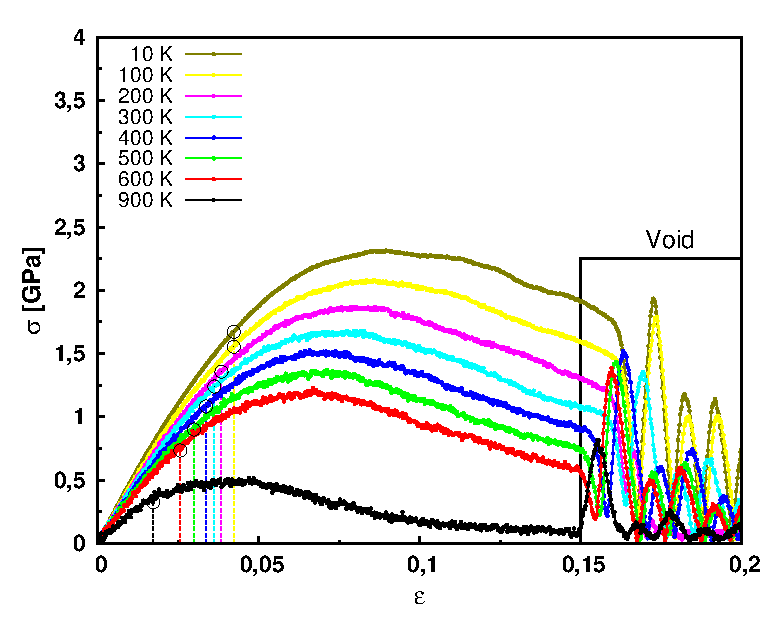
\includegraphics[width=6.3cm]{Presentacion_Mecom_2012/Tens_stress_strain_curve.eps}}
	\subfloat[Compresi\'on]{
	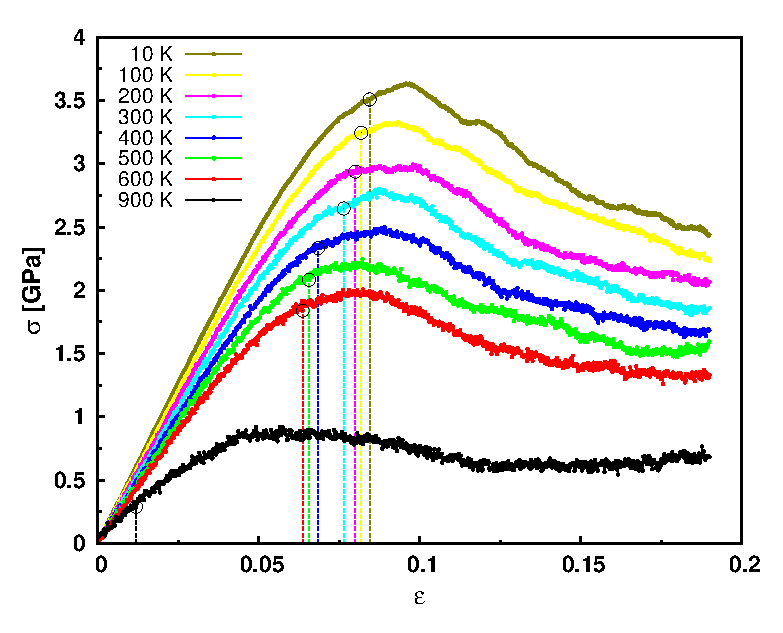
\includegraphics[width=6.3cm]{Presentacion_Mecom_2012/Comp_stress_strain_curve.eps}}
      \end{figure}
    \end{textblock*}
    \begin{textblock*}{6cm}(3.5cm,8cm) 
    \centering
      Tg=696 K\\
      (Glass transition temperature)
    \end{textblock*}
\end{frame}

\begin{frame}
 \frametitle{Resultados de las aproximaciones}
 \begin{textblock*}{6cm}(0.5cm,1.5cm) 
    
    \begin{table}[htp]
    \begin{center}
    \begin{tabular}{c c}
    \hline
    \textbf{Tracci\'on} & $R^{2}$ \\ \hline \hline
    Peak Von Mises stress &  0.981 \\ \hline
    Von Mises stress ($\epsilon=0.12$) & 0.998 \\ \hline
    Young Modulus & 0.990 \\ \hline
    Yield Stress &  0.972 \\ \hline
    \end{tabular}
    \end{center}
    \end{table}

    \begin{table}[htp]
    \begin{center}
    \begin{tabular}{*{4}{c}}
    \hline
    \textbf{Compresi\'on} & $R^{2}$ \\ \hline \hline
    Peak Von Mises stress & 0.997 \\ \hline
    Von Mises stress ($\epsilon=0.18$) & 0.972 \\ \hline
    Young Modulus & 0.985 \\ \hline
    Yield Stress & 0.985 \\ \hline
    \end{tabular}
    \end{center}
    \end{table}
 \end{textblock*}
  \begin{textblock*}{4.8cm}(7.7cm,2cm)
  \centering
   Para el c\'alculo de propiedades mec\'anicas, suponemos un comportamiento activado t\'ermicamente.
    $y=A_1^{(-T/T_0)}$
  \end{textblock*}
  \begin{textblock*}{4.8cm}(7.7cm,6cm)
  \centering
   El coeficiente de correlaci\'on es mayor a 0.9 en todos los casos, lo cual demuestra que la ecuaci\'on propuesta es razonable.
  \end{textblock*}
\end{frame}

\begin{frame}
 \frametitle{Gr\'aficos de las aproximaciones}
 \begin{textblock*}{10cm}(1.5cm,1cm)
 \begin{figure}[htp]
    \centering
    \includegraphics[width=5cm]{Presentacion_Mecom_2012/young_T_both.eps}
    \includegraphics[width=5cm]{Presentacion_Mecom_2012/peakstress_T_BOTH.eps}
  \end{figure} 
 \end{textblock*}
 \begin{textblock*}{5cm}(1.5cm,4.9cm)
   \begin{figure}[htp]
    \centering
    \includegraphics[width=5cm]{Presentacion_Mecom_2012/defstress_T_BOTH.eps}
  \end{figure} 
 \end{textblock*}
 \begin{textblock*}{5cm}(6.8cm,6.7cm)
  \centering
   Disminuci\'on de los valores con el aumento de temperatura.
  \end{textblock*}
\end{frame}

\begin{frame}
 \frametitle{Formaci\'on del void}
 \begin{figure}
    \centering
    \begin{tabular}{C{5cm} c}
      \includegraphics[width=5cm]{Cap_3/Poro_900_94000light_100-400.png} &  \multirow{3}{*}{\includegraphics[width=1.2cm]{Cap_3/scale.png}}\\
      \includegraphics[width=5cm]{Cap_3/Poro_900_96000light_100-400.png} & \\
      \includegraphics[width=5cm]{Cap_3/Poro_900_98000light_100-400.png} & \\
    \end{tabular}
    \label{C3:fg:voidSeq}
  \end{figure}
  \begin{textblock*}{2cm}(1cm,3cm)
      $\epsilon=14.4\%$
  \end{textblock*}
  \begin{textblock*}{2cm}(1cm,5.5cm)
    $\epsilon=14.6\%$
  \end{textblock*}
  \begin{textblock*}{2cm}(1cm,8cm)
    $\epsilon=14.8\%$
  \end{textblock*}
  \begin{textblock*}{4cm}(8.5cm,2.5cm)
    Temperatura 900K
  \end{textblock*}
\end{frame}

\begin{frame}
 \frametitle{Comportamiento pl\'astico}
 \begin{textblock*}{7cm}(0.5cm,1.4cm)
  \begin{figure}[htp]
      \centering
      \includegraphics[width=7cm]{Presentacion_Mecom_2012/Fit2_Tercios.png}
  \end{figure}
 \end{textblock*}
 \begin{textblock*}{4.5cm}(8cm,2.5cm)
      Expresi\'on adaptada de Cheng et al. (2011) :\\
	$\sigma_y/G =A+B(T/T_g)^{2/3}$
  \end{textblock*}
  \begin{textblock*}{4.5cm}(8cm,4.5cm)
      Valores normalizados mediante:
      \begin{itemize}
       \item $T_g=696K$
       \item $G=30GPa$
      \end{itemize}
      (Johnson y Samwer, 2005)
  \end{textblock*}
  \begin{textblock*}{5cm}(2cm,6.5cm)
    \scriptsize{Esfuerzo de fluencia vs. temperatura}
  \end{textblock*}
  \begin{textblock*}{12cm}(0.5cm,8.5cm) % {block width} (coords)
    \scriptsize{Cheng Y.Q. and Ma E.. Acta Mater., 59, 1800-1807 (2011).\\
    Johnson W.L., Samwer K.. Phys. Rev. Lett., 95, 195501 (2005).}
  \end{textblock*}
\end{frame}

\begin{frame}
  \frametitle{Muestras}
  \begin{textblock*}{6cm}(0.5cm,1.5cm)
    \begin{figure}[htp]
      \centering
      \includegraphics[width=6cm]{Cap_3/All_300K_6pstrain_sacale100-280_Trac.png}
    \end{figure}
  \end{textblock*}
  \begin{textblock*}{6cm}(6.5cm,4cm)
    \begin{figure}[htp]
      \centering
      \includegraphics[width=6cm]{Cap_3/All_300K_6pstrain_sacale100-400_Comp.png}
    \end{figure}
  \end{textblock*}
  \begin{textblock*}{4cm}(3cm,6.2cm)
   \scriptsize{Tracci\'on. $T=300K$. $\epsilon=6\%$}
  \end{textblock*}
  \begin{textblock*}{5cm}(8cm,8.5cm)
   \scriptsize{Compresi\'on. $T=300K$. $\epsilon=6\%$}
  \end{textblock*}
  \begin{textblock*}{5cm}(7cm,2.5cm)
   \centering
   La escala de colores representa la tensi\'on de Von Mises
  \end{textblock*}
  \begin{textblock*}{5cm}(1cm,7.5cm)
   \centering
   No se observan bandas de corte
  \end{textblock*}
\end{frame}

\begin{frame}
  \frametitle{Deformaci\'on at\'omica}
  \begin{textblock*}{4cm}(4.5cm,1.5cm)
    \begin{figure}[htp]
      \centering
      \includegraphics[height=6cm]{Cap_3/ShearBand.png}
    \end{figure}
  \end{textblock*}
  \begin{textblock*}{5cm}(6.5cm,8.5cm)
   \scriptsize{Compresi\'on. $T=300K$. $\epsilon=14\%$}
  \end{textblock*}
  \begin{textblock*}{5cm}(0.5cm,3cm)
   \centering
   La escala de colores representa deformaci\'on at\'omica
  \end{textblock*}
  \begin{textblock*}{5cm}(0.5cm,5.5cm)
   \centering
   Hay bandas de corte incipientes que se forman con una direcci\'on predominantemente diagonal
  \end{textblock*}
  
\end{frame}

\begin{frame}
  \frametitle{Resultados bajo condiciones libres}
  
  \begin{textblock*}{5cm}(0.5cm,1.2cm)
    \begin{figure}[htp]
      \centering
      \includegraphics[width=5cm]{Cap_3/Pseudo_Free_Boundaries_ShearStrain_0_035_300K_20strain.png}
    \end{figure}
  \end{textblock*}
  
  \only<1>{
  \begin{textblock*}{5cm}(6.5cm,1.2cm)
    \begin{figure}[htp]
      \centering
      \includegraphics[width=5cm]{Cap_3/Pseudo_Free_Boundaries_ShearStrain_005_046_300K_15strain.png}
    \end{figure}
  \end{textblock*}
  }
  
  \begin{textblock*}{4cm}(2.3cm,5.5cm)
   \scriptsize{Tracci\'on. $T=300K$. $\epsilon=20\%$}
  \end{textblock*}
  
  \only<1>{
  \begin{textblock*}{4cm}(8.7cm,5.5cm)
   \centering
   \scriptsize{Compresi\'on. $T=300K$. $\epsilon=15\%$}
  \end{textblock*}
  }
  
  \begin{textblock*}{6cm}(0.2cm,6.5cm)
   \centering
   Hay cambio de la secci\'on transversal en tracci\'on.\\
   Son similares a las de nanoalambres de vidrios met\'alicos vistas en Xiao et al. (2012).\\
  \end{textblock*}
  
  \only<1>{
  \begin{textblock*}{3cm}(6cm,5.5cm)
    \begin{figure}[htp]
	\includegraphics[width=1.3cm]{Cap_3/Pseudo_Free_Boundaries_0strain_transversal.png}
	\includegraphics[width=1.3cm]{Cap_3/Pseudo_Free_Boundaries_20strain_transversal_esquina.png}
    \end{figure}
  \end{textblock*}
  }
  
  \only<2>{
  \begin{textblock*}{2cm}(8.7cm,1.8cm)
    \begin{figure}[htp]
	\includegraphics[width=2cm]{Presentacion_Mecom_2012/XiaoNanowire.png}
    \end{figure}
  \end{textblock*}
  
  \begin{textblock*}{6cm}(6cm,8.2cm)
    \centering
    \scriptsize{Xiao Q., Sheng H.W. and Shi Y.. MRS Communications, 2, 13-16 (2012)}
  \end{textblock*}

  \begin{textblock*}{2cm}(6.7cm,3.1cm)
    \centering
    \scriptsize{$1.7\cdot10^{12}K/s$}
  \end{textblock*}
  
  \begin{textblock*}{2cm}(6.7cm,4.9cm)
    \centering
    \scriptsize{$1.7\cdot10^{11}K/s$}
  \end{textblock*}
  
  \begin{textblock*}{2cm}(6.7cm,6.8cm)
    \centering
    \scriptsize{$1.7\cdot10^{10}K/s$}
  \end{textblock*}
  
  }
\end{frame}
%%%%%%%%%%%%%%%%%%%%%%%%%%%%%%%%%%%%%%%%%%%%%%%%%%%%%
%		CAP 4
%%%%%%%%%%%%%%%%%%%%%%%%%%%%%%%%%%%%%%%%%%%%%%%%%%%%%

\section[BMG con nanopart\'iculas]{BMG con nanopart\'iculas embebidas}
%\subsection{BMG con nanopart\'iculas embebidas}

\begin{frame}
  \frametitle{Introducción}
  \begin{itemize}
   \item La plasticidad es dominada por STZs que crecen y colapsan en SBs las cuales conducen a una falla frágil del material.
   \item Para homogeneizar el régimen plástico y evitar esto, la composición se modifica de diferentes maneras
  \end{itemize}
  \vspace{-1cm}
  \begin{figure}[htp]
    \centering
    \begin{tabular}{c}
      \subfloat[Nano partículas \cite{Albe13}]{
	      \includegraphics[width=5cm]{../Figures/Presentacion/nanoparticles_example.png}
	      \label{P:fg:B2Crystal}}
    \quad
      \subfloat[Nano vidrios \cite{Adibi13}]{
	      \includegraphics[width=5cm]{../Figures/Presentacion/nanoglass_example.png}
	      \label{P:fg:B2CrystalTest}}
    \end{tabular}
    \caption{BMGs con composición modificada}
    \label{P:fg:B2CuZr_Formation}
  \end{figure} 
\end{frame}

\begin{frame}
Se estudia:
 \begin{itemize}
  \item Estabilidad térmica de las nanopartículas (difusión del material cristalino en la matriz amorfa).
  \item Impacto en el comportamiento mecánico de la muestra (cambios en curvas tensión-deformación)
  \item Distribución de la tensión de corte en la muestra.
 \end{itemize}
\end{frame}

%%%%%%%%%%%%%%%%%%%%%%%%%%%%%%%%%%%%%%%%%%%%%%%%%%%%%
%		CAP 5
%%%%%%%%%%%%%%%%%%%%%%%%%%%%%%%%%%%%%%%%%%%%%%%%%%%%%

\section[BMG poroso]{BMG poroso sinterizado}
\subsection{BMG poroso sinterizado}
%%%
% Introduccion
%%%

\begin{frame}
    \frametitle{Introducci\'on}
    \vspace{0.2cm}
%    \begin{itemize}
%        \item Metallic Glass: amorphous metal (without crystalline order).
%        \item Has advantages over crystalline metals, like elasticity combined with high resistance, strength and moldability.
%        \item Plasticity in these materials occurs by nucleation of shear transformation zones which grow into shear bands.
%        \item Shear bands may lead to brittle failure (heterogeneous deformation): importance of \textbf{preventing their propagation}.
%        \item A more homogeneous deformation may be achieved by adding \textbf{porosity}.
%    \end{itemize} 
    \begin{block}{Problem\'atica}
      Las bandas de corte pueden ocasionar la falla fr\'agil del material (deformaci\'on heterog\'enea)
    \end{block}
    \begin{block}{Posible soluci\'on}
     Una deformaci\'on m\'as homog\'enea puede lograrse al agregar porosidad\\
     Similar al bloqueo del deslizamiento en metales cristalinos
    \end{block}
\end{frame}

%%%
% Preparacion de la muestra
%%%

\begin{frame}
    \frametitle{Preparaci\'on de la muestra porosa}
    \vspace{0cm}
    \begin{enumerate}
        \item Ubicaci\'on aleatoria de part\'iculas de 2.5 nm de radio.
        \item Relajaci\'on @ 650K (volumen constante, pocos ps). 
        \item Hasta 10 ps de compresi\'on (400 bar).
        \item Se repiten los dos pasos anteriores.
        \item M\'as relajaci\'on: enfriado a temperatura 0, bar\'ostato a presi\'on 0, calentado hasta temperatura de simulaci\'on y bar\'ostato a presi\'on 0 (5 ps, temperatura constante)
        \begin{textblock*}{3cm}(2.5cm,6.5cm) % {block width} (coords)
            \includegraphics[width=3cm]{Cap_5/spheres2.png}
        \end{textblock*}
        \begin{textblock*}{3cm}(7cm,6.5cm) % {block width} (coords)
            \includegraphics[width=3cm]{Cap_5/spheres3.png}
        \end{textblock*}
    \end{enumerate}
\end{frame}

%%%
% Resultados
%%%

\begin{frame}
    \frametitle{Detalles de la simulaci\'on}
    \vspace{0cm}
    \begin{itemize}
        \item Se crearon muestras con distintos niveles de porosidad (3.3\%, 5.8\% y 13.1\%).
        \item Velocidad de deformaci\'on 10$^9/s$, deformaci\'on puramente uniaxial.
        \item Condiciones de borde peri\'odicas.
    \end{itemize}
    \begin{textblock*}{12cm}(0.5cm,5cm)
      \begin{figure}[htp]
	\includegraphics[width=4cm]{Cap_5/3_0strain.png}
	\includegraphics[width=4cm]{Cap_5/6_0strain.png}
	\includegraphics[width=4cm]{Cap_5/13_0strain_pores.png}
      \end{figure}
    \end{textblock*}
\end{frame}

\begin{frame}
 \frametitle{Resultados}
 \begin{textblock*}{12cm}(0.5cm,1.5cm)
  \begin{figure}[htp]
      \includegraphics[width=6cm]{Cap_5/SVF_strain_comp_dash.eps}
      \includegraphics[width=6cm]{Cap_5/SVF_strain_tens.eps}
  \end{figure}
 \end{textblock*}
 \begin{textblock*}{6cm}(0.8cm,7cm)
  \centering
  \scriptsize{Compresi\'on}
 \end{textblock*}
 \begin{textblock*}{6cm}(6.8cm,7cm)
  \centering
  \scriptsize{Tracci\'on}
 \end{textblock*}
  \begin{textblock*}{\textwidth}(1cm,7.7cm)
  \centering
  Fracci\'on de volumen s\'olido vs deformaci\'on.\\
  El uso de condiciones peri\'odicas evita el cierre de poros en tracci\'on.
 \end{textblock*}
\end{frame}


\begin{frame}
    \frametitle{Resultados (compresi\'on)}
    \begin{textblock*}{7cm}(5.5cm,2cm) % {block width} (coords)
        \includegraphics[width=7cm]{Presentacion_PANACM_Franco/Pzz_strain_comp_dash.eps}
    \end{textblock*}
    \begin{textblock*}{4.2cm}(5.8cm,6.4cm) % {block width} (coords)
        \begin{tikzpicture}
            \draw[thick] (0,0) rectangle (5cm,1.2cm);
        \end{tikzpicture}
    \end{textblock*}
    \begin{textblock*}{5cm}(0.6cm,2.2cm) % {block width} (coords)
        Los poros act\'uan como concentradores de tensi\'on, promoviendo la plasticidad. %Previo al colapso de los poros, la deformaci\'on aumenta, manteniendo bajos niveles de tensi\'on.
    \end{textblock*}
    \begin{textblock*}{4.5cm}(0.6cm,5cm) % {block width} (coords)
        Luego del colapso de los poros hay un endurecimiento significativo. %Indicar que todas las curvas son iguales
    \end{textblock*}
    \begin{textblock*}{12cm}(0.6cm,8.5cm) % {block width} (coords)
        A mayor porosidad $\rightarrow$ menor esfuerzo para cerrar los poros
    \end{textblock*}
\end{frame}

\begin{frame}
    \frametitle{Resultados (compresi\'on)}
    \begin{textblock*}{7cm}(5.5cm,2cm)
        \includegraphics[width=7cm]{Presentacion_PANACM_Franco/tipe3_strain_comp.eps}
    \end{textblock*}
    \begin{textblock*}{4.8cm}(0.5cm,2.2cm)
        La ca\'ida en el n\'umero de \'atomos de Tipo 3 luego de una etapa constante ha sido considerada como un indicador del inicio de la plasticidad (Arman, 2010).
    \end{textblock*}
    \begin{textblock*}{4.8cm}(0.5cm,6.5cm)
        El resultado es contra-intuitivo.\\%Hay plasticidad pero los poliedros de Voronoi pr\'acticamente no cambian.\\
        Posible que hayan otros procesos involucrados.
    \end{textblock*}
\end{frame}

\begin{frame}
    \frametitle{Resultados (compresi\'on)}
    \begin{textblock*}{12cm}(0.4cm,1.7cm)
        \includegraphics[width=4cm]{Cap_5/13_0strain.png}
        \includegraphics[width=4cm]{Cap_5/13_5strain_comp.png}
        \includegraphics[width=4cm]{Cap_5/13_12strain_comp.png}\\
    \end{textblock*}
    \begin{textblock*}{12cm}(0.4cm,5.4cm)
     \centering
        \includegraphics[width=4cm]{Cap_5/escala.png}
    \end{textblock*}
    \begin{textblock*}{12cm}(0.5cm,6.2cm)
        \centering
        \scriptsize{Porosidad 13\%. $\epsilon=$ 0, 5 y 12\%, respectivamente.}
    \end{textblock*}
    \begin{textblock*}{11cm}(1cm,7.1cm)
      \centering
        %Los poros act\'uan como concentradores de tensiones.\\
        Los poros impiden la propagaci\'on de bandas de corte.\\
        Bandas de corte nuclean diagonalmente en el espacio entre poros.
    \end{textblock*}
\end{frame}

\begin{frame}
    \frametitle{Resultados (tracci\'on)}
    \begin{textblock*}{7cm}(0.4cm,2cm) % {block width} (coords)
        \includegraphics[width=7cm]{Cap_5/Pzz_strain_tens.eps}
    \end{textblock*}
    \begin{textblock*}{4cm}(8cm,2.2cm) % {block width} (coords)
        \includegraphics[width=4cm]{Presentacion_PANACM_Franco/13_20strain_tens_2.png}\\
        \centering
        \scriptsize{Deformaci\'on at\'omica.\\Porosidad 13\%, deformaci\'on 20\%.}
    \end{textblock*}
    \begin{textblock*}{11.5cm}(0.5cm,7.8cm) % {block width} (coords)
	\centering
        Flujo pl\'astico.\\
        El uso de condiciones de borde peri\'odicas evita el cierre de poros (no hay estricci\'on).
    \end{textblock*}
\end{frame}

\begin{frame}
    \frametitle{Resultados (tracci\'on)}
    \begin{textblock*}{12cm}(0.4cm,2cm) % {block width} (coords)
        \includegraphics[width=4cm]{Presentacion_PANACM_Franco/13_0strain.png}
        \includegraphics[width=4cm]{Presentacion_PANACM_Franco/13_6strain_tens.png}
        \includegraphics[width=4cm]{Presentacion_PANACM_Franco/13_20strain_tens_2.png}
    \end{textblock*}
    \begin{textblock*}{12cm}(0.4cm,6.9cm)
     \centering
        \includegraphics[width=4cm]{Cap_5/escala.png}
    \end{textblock*}
    \begin{textblock*}{12cm}(0.5cm,7.7cm)
        \centering
        \scriptsize{Porosidad 13\%. $\epsilon=$ 0, 6 y 20\%, respectivamente.}
    \end{textblock*}
    \begin{textblock*}{11.5cm}(1cm,8.5cm) % {block width} (coords)
    \centering
	La deformaci\'on cortante se concentra principalmente alrededor de los poros.
%            \item Relative position between atoms remains almost the same.
    \end{textblock*}
\end{frame}

\begin{frame}
    \frametitle{Resultados (tracci\'on)}
    \begin{textblock*}{7.5cm}(0.3cm,2cm) % {block width} (coords)
        \includegraphics[width=7.5cm]{Presentacion_PANACM_Franco/tipe3_strain_tens.eps}
    \end{textblock*}
    \begin{textblock*}{4.2cm}(6.7cm,4cm) % {block width} (coords)
        \begin{tikzpicture}
            \draw[thick] (0,0) rectangle (1.4cm,2cm);
        \end{tikzpicture}
    \end{textblock*}
    \begin{textblock*}{5cm}(8cm,3cm) % {block width} (coords)
        Constante luego de la nucleaci\'on del void.
    \end{textblock*}
    \begin{textblock*}{12cm}(0.4cm,7.9cm) % {block width} (coords)
    \centering
	Se facilita el movimiento de \'atomos alrededor de los poros.\\
	Esto evita la formaci\'on de STZ fuera de los alrededores de los poros.
    \end{textblock*}
\end{frame}

%%%
% Conclusiones
%%%

%\begin{frame}
    %\frametitle{Conclusions}
    %\vspace{0.5cm}
    %\begin{itemize}
        %\item Sintering process leads to glass with taylored porosity values.
        %\item Under compression: pores act as stress concentrators but also delay nucleation of SBs. After closure, there is hardening.
        %\item Under tension: pores do not close and they concentrate plastic flow around them, also impeding formation of STZ and SBs.
        %\item Results under strain were somewhat comparable to the ones by Yuan et al. (2014), where a single crystal sample with voids was studied.
    %\end{itemize}
    %\begin{textblock*}{12cm}(1cm,8.8cm) % {block width} (coords)
        %\scriptsize{Yuan F. and Wu X., \textit{AIP ADVANCES}, \textbf{4}, 127109 (2014).}
    %\end{textblock*}
%\end{frame}

%\begin{frame}
    %\begin{textblock*}{5cm}(2cm,3.2cm) % {block width} (coords)
        %\includegraphics[width=5cm]{Presentacion_PANACM_Franco/stress_strain_comp_dash.eps}
    %\end{textblock*}
    %\begin{textblock*}{3cm}(7cm,3cm) % {block width} (coords)
        %\includegraphics[width=5cm]{Presentacion_PANACM_Franco/Yuan_VM.png}
    %\end{textblock*}
    %\begin{textblock*}{12cm}(1cm,8.2cm) % {block width} (coords)
        %\small{Yuan F. and Wu X., \textit{AIP ADVANCES}, \textbf{4}, 127109 (2014).}
    %\end{textblock*}
%\end{frame}

%\begin{frame}
    %\begin{textblock*}{5cm}(2cm,3.2cm) % {block width} (coords)
        %\includegraphics[width=5cm]{Presentacion_PANACM_Franco/SVF_strain_comp_dash.eps}
    %\end{textblock*}
    %\begin{textblock*}{3cm}(7cm,3cm) % {block width} (coords)
        %\includegraphics[width=5cm]{Presentacion_PANACM_Franco/Yuan_SVF.png}
    %\end{textblock*}
    %\begin{textblock*}{12cm}(1cm,8.2cm) % {block width} (coords)
        %\small{Yuan F. and Wu X., \textit{AIP ADVANCES}, \textbf{4}, 127109 (2014).}
    %\end{textblock*}
%\end{frame}

\begin{frame}
 \frametitle{Influencia velocidad de enfriamiento}
\end{frame}

\begin{frame}
 \frametitle{Influencia ubicaci\'on de poros}
\end{frame}

%%%%%%%%%%%%%%%%%%%%%%%%%%%%%%%%%%%%%%%%%%%%%%%%%%%%%
%		APENDICES
%%%%%%%%%%%%%%%%%%%%%%%%%%%%%%%%%%%%%%%%%%%%%%%%%%%%%

\section{Trabajo computacional}
%\subsection{Trabajo computacional}

\begin{frame}
 
\end{frame}
%%%%%%%%%%%%%%%%%%%%%%%%%%%%%%%%%%%%%%%%%%%%%%%%%%%%%
%		CONCLUSIONES
%%%%%%%%%%%%%%%%%%%%%%%%%%%%%%%%%%%%%%%%%%%%%%%%%%%%%

\section{Conclusiones}
%\subsection{Conclusiones}

\begin{frame}
 
\end{frame}

\section{Bibliografía}
\begin{frame}
  \tiny{\bibliographystyle{apalike}}
  \bibliography{../Bibliography}
\end{frame}

%%%
% Slide de titulo
%%%

\maketitle

\end{document}
